\documentclass{article}

% Language setting
% Replace `english' with e.g. `spanish' to change the document language
\usepackage[french]{babel}
\usepackage[fleqn]{amsmath} % Aligner les équations à gauche


% Set page size and margins
% Replace `letterpaper' with`a4paper' for UK/EU standard size
\usepackage[letterpaper,top=2cm,bottom=2cm,left=3cm,right=3cm,marginparwidth=1.75cm]{geometry}

% Useful packages

\usepackage{amsmath}
\usepackage{graphicx}
\usepackage{subcaption}
\usepackage[colorlinks=true, allcolors=blue]{hyperref}

\title{TD 5 - Electromagnétisme}
\author{IPESUP - PC }
\date{09/10/2024}

\begin{document}
\maketitle

\section{Rappels de cours}

Equations de Maxwell statiques locales:\\
\begin{align*}
    div(\vec{E}) &= \frac{\rho}{\varepsilon_0} \\
    rot(\vec{E}) &= 0 \\
    div(\vec{B}) &= 0 \\
    rot(\vec{B}) &= \mu_0 \vec{j}
\end{align*}

Equations de Maxwell statiques globales:\\

\begin{align*}
    &\oint_S \vec{E} \cdot d\vec{S} = \frac{Q_{int}}{\varepsilon_0} \\
    &\oint_S \vec{B} \cdot d\vec{S} = 0 \\
    &\oint_\Gamma \vec{E} \cdot d\vec{l} = 0 \\
    &\oint_\Gamma \vec{B} \cdot d\vec{l} = \mu_0 I_{int}
\end{align*}



\section{Exercice 1: }






\begin{figure}[h]
  \centering
  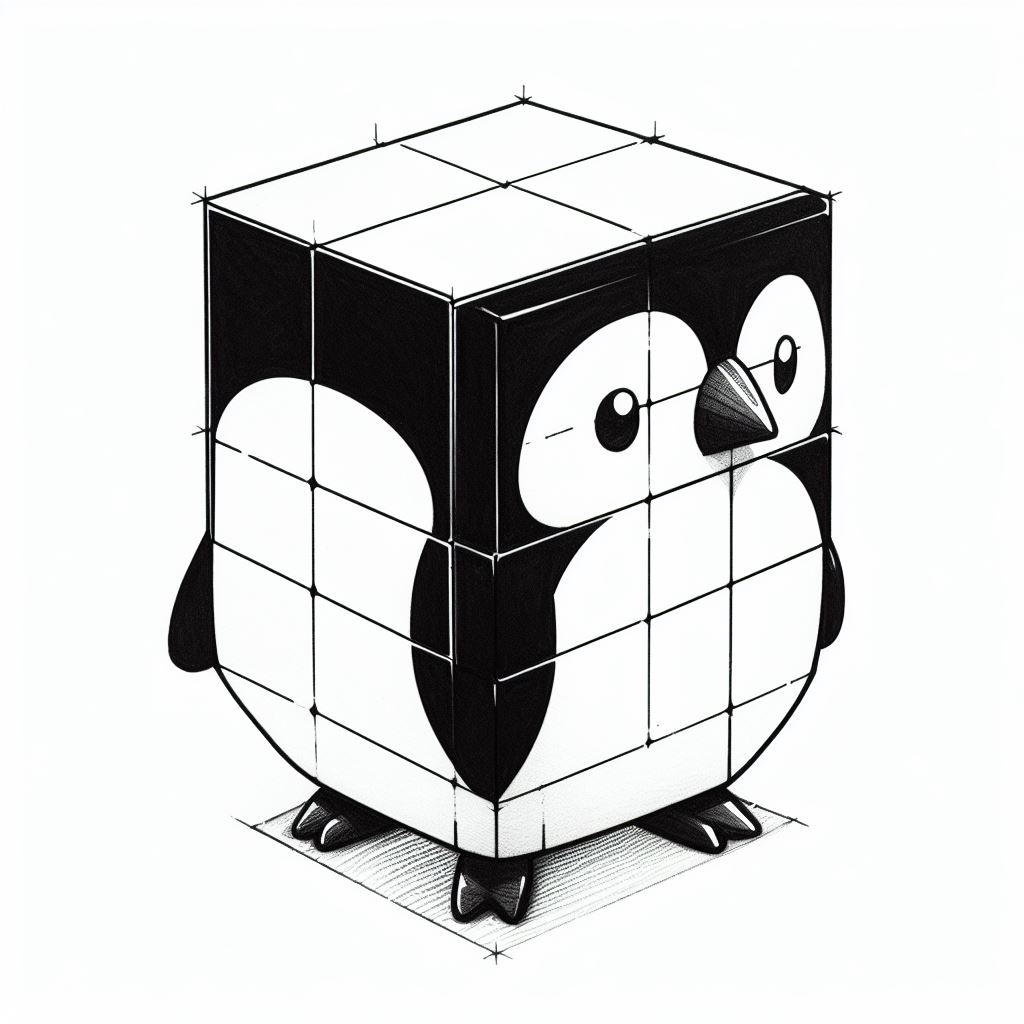
\includegraphics[width=0.4\textwidth]{pingouin_schema.jpeg}
  \label{fig:maison}
    \caption{MA FIGURE}
\end{figure}



\end{document}

